\section{实数集与欧氏空间中的邻域和闭区间}
\label{sec:analysis-metric-measurement}
\label{sec:analysis-set-metric}

前两节的数列极限与函数极限都在控制距离：$|a_n-a|<\varepsilon$说明第$n$项离极限不远，
$0<|x-a|<\delta$说明输入离中心不远。本节先在实轴和有限维欧氏空间中把“一个点附近”写成开球与邻域，
再用邻域定义开集、闭集，并用点列刻画闭性；最后建立闭区间的有限子覆盖性质。
这些结论直接服务于下一章一元函数的连续性和极值，也服务于多元微积分中的欧氏集合。
把绝对值和欧氏范数抽象成任意集合上的度量，再讨论一般空间的完备性、可分性、全有界和紧致序列刻画，
是第~\ref{chap:metric-spaces}章“度量空间”的任务；本节不预设一般度量空间的结论。

\subsection{开球、邻域与开闭集}

\paragraph{开球与邻域}
讨论一个点附近的变化，需要先指定哪些对象算作离它足够近。给定中心和距离阈值后，可以把这些对象收集成一个集合。

\begin{definition}[欧氏开球]
\label{def:analysis-open-ball}
在$\mathbb R^d$中，以$\bm{x}$为中心、半径$r>0$的\term{开球}（open ball）记为
$B(\bm{x},r)=\{\bm{y}\in\mathbb R^d:\lVert\bm{y}-\bm{x}\rVert_2<r\}$。
当$d=1$时，$B(x,r)=(x-r,x+r)$就是开区间。
\end{definition}

开球把“离一个点足够近”写成集合。若集合$V$包含某个$B(\bm{x},r)$，就称$V$是$\bm{x}$的邻域；
邻域本身不必是开集。由这些邻域可以判断一个范围是否包含其中每个点附近的点。

图~\ref{fig:analysis-ball-neighborhood}将这两个对象分开：开球由距离直接确定，邻域则只需包含一个这样的开球。
\begin{figure}[htbp]
 \centering
 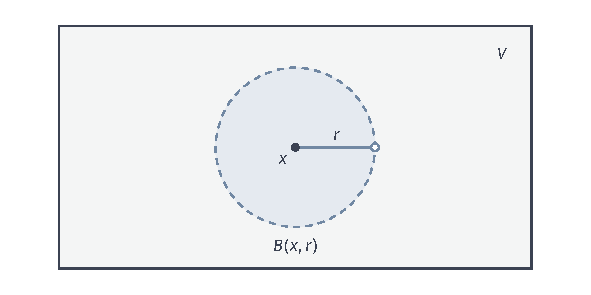
\includegraphics[width=\linewidth]{figures/01-mathematical-preliminaries-upper/01-mathematical-language-combinatorics-analysis-optimization/tikz/metric-ball-neighborhood/figure.pdf}
 \caption{平面欧氏距离下的开球与邻域。浅蓝圆盘为$B(\bm{x},r)$，虚线圆周不属于开球；灰色矩形$V$连同实线边界包含这个圆盘，因此是$\bm{x}$的邻域。$V$本身不是开集，说明“是某点的邻域”只要求在该点周围留有余量。}
 \label{fig:analysis-ball-neighborhood}
\end{figure}

\paragraph{开集与闭集}
有了开球，就能检验一个集合是否容纳其中每个点附近的一小片范围。对集合的补集作同样检验，又得到另一类常用的范围条件。

\begin{definition}[开集与闭集]
\label{def:analysis-open-closed-sets}
在$\mathbb R^d$中，集合$U$若对每个$\bm{x}\in U$都存在$r>0$使$B(\bm{x},r)\subseteq U$，就称为\term{开集}（open set）；
集合$F$若其补集$\mathbb R^d\setminus F$为开集，就称为\term{闭集}（closed set）。
\end{definition}

开闭性总是相对于当前空间而言。例如$[0,1/2)$在$\mathbb R$中不是开集，
但在子空间$X=[0,1]$中是开集：此时开球是实轴开区间与$X$的交，
$0$的一个小球不必包含负数。全集和空集既开又闭；“不是开集”也不等于“就是闭集”，实轴上的$[0,1)$便两者都不是。

图~\ref{fig:analysis-open-closed-relative}用端点附近的小球检验上述区别：实轴上包含端点的区间可能无法容纳小球，而在子空间中，小球本身也会随空间改变。
\begin{figure*}[htbp]
 \centering
 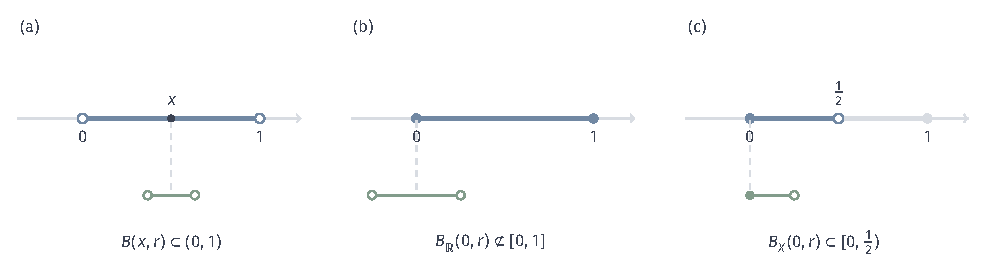
\includegraphics[width=169mm]{figures/01-mathematical-preliminaries-upper/01-mathematical-language-combinatorics-analysis-optimization/tikz/metric-open-closed-relative/figure.pdf}
 \caption{开集、闭集与所在空间。蓝色线段为待检验集合，绿色线段示意小球，空心端点排除、实心端点包含。(a) 在$\mathbb R$中，$(0,1)$的每个点都能选取一个包含于集合的小球，故为开集。(b) $[0,1]$在端点$0$处不能容纳任何实轴小球，因而不是开集；其补集$(-\infty,0)\cup(1,\infty)$为开集，故它是闭集。(c) 改在$X=[0,1]$中取球时，$B_X(0,r)=[0,r)$（$0<r<1/2$），因此$[0,1/2)$是$X$中的开集。图中只画出(c)的端点检验，其余点可直接沿用区间内部的小球。}
 \label{fig:analysis-open-closed-relative}
\end{figure*}

开球本身确实是开集：若$\bm{y}\in B(\bm{x},r)$，取$\rho=r-\lVert\bm{y}-\bm{x}\rVert_2>0$，
则三角不等式保证$B(\bm{y},\rho)\subseteq B(\bm{x},r)$。
任意多个开集的并仍开，因为并集中每个点都已属于某一个开集，可以沿用它的小球；
有限个开集的交仍开，因为可取各个允许半径的最小值。
无限多个开集的交则未必开，例如$\bigcap_{n\geq1}(-1/n,1/n)=\{0\}$。

\subsection{闭集的序列判据}

在欧氏空间中，闭集也可以用点列极限是否留在集合内来刻画。
$\mathbb R^d$中的点列$(\bm{x}_n)$收敛到$\bm{x}$，是指$\lVert\bm{x}_n-\bm{x}\rVert_2\to0$；
由于
\[
  |x_{n,j}-x_j|\leq\lVert\bm{x}_n-\bm{x}\rVert_2
  \leq\sqrt d\max_{1\leq j\leq d}|x_{n,j}-x_j|,
\]
欧氏距离收敛与有限个坐标同时收敛等价。

\begin{lemma}[闭集的序列判据]
\label{lem:analysis-closed-sequence-criterion}
设$F$为$\mathbb R^d$中的集合。$F$是闭集，当且仅当：对每个取值于$F$的点列$(\bm{x}_n)$，
若$\bm{x}_n\to\bm{x}$在$\mathbb R^d$中成立，则$\bm{x}\in F$。
\end{lemma}
\begin{proof}
若$F$闭而$\bm{x}\notin F$，开集$\mathbb R^d\setminus F$包含某个$B(\bm{x},r)$。
收敛要求充分靠后的$\bm{x}_n$落入这个球，与$\bm{x}_n\in F$矛盾。
反之，若$F$不闭，则存在$\bm{x}\in\mathbb R^d\setminus F$，使每个$B(\bm{x},r)$都与$F$相交。
为每个$n$选$\bm{x}_n\in F\cap B(\bm{x},1/n)$，便有$\bm{x}_n\to\bm{x}\notin F$，违反序列条件。
\end{proof}

例如$(0,1)$中的$1/n$在$\mathbb R$中趋于$0$，而$0\notin(0,1)$，所以$(0,1)$不是实轴中的闭集；
改在子空间$(0,1)$中判断时，$0$已不是环境中的候选极限。闭与有界描述的也是不同性质：
$(0,1)$有界但不闭，$\mathbb R$闭但不有界。

\subsection{闭区间的有限子覆盖性质}

\paragraph{开覆盖与有限子覆盖}

连续性在每一点给出一个邻域内的控制，但不同点的邻域大小可能不同。
要得到对整个闭区间同时有效的结论，需要从无限多个邻域中选出有限个，仍覆盖整个区间；
测量区间长度时也会遇到同样的问题：用可数多个开区间覆盖闭区间后，希望只保留其中有限个。
下面先规定“从一族开集中选出有限部分仍不遗漏”的含义。
\begin{definition}[开覆盖与紧致性]
\label{def:analysis-compactness}
设$K\subseteq\mathbb R^d$。一族开集的并包含$K$时，称它们为$K$的\term{开覆盖}（open cover）；
从中选出的有限个开集仍覆盖$K$时，称它们构成\term{有限子覆盖}（finite subcover）。
若$K$的每个开覆盖都存在有限子覆盖，则称$K$\term{紧致}（compact）。
\end{definition}
开覆盖本身可以有无限多个成员；有限子覆盖要求从原来的成员中挑选，而不是另换一组集合。

\paragraph{闭区间的紧致性}

闭区间里的点不会逃向无穷，收敛子列的极限也不会离开区间。
这两个条件使局部邻域覆盖不能一直要求加入新的成员。
\begin{theorem}[闭区间的有限子覆盖性质]
\label{thm:analysis-interval-finite-subcover}
实轴上的每个闭区间$[a,b]$都是紧致集。
\end{theorem}
\begin{proof}
$a=b$时选择一个包含该点的覆盖成员即可。设$a<b$，并给定$[a,b]$的开覆盖$\mathcal U$。
先证明这组覆盖有一个共同尺度：
\begin{equation}
 \exists r>0,\quad\forall x\in[a,b],\quad\exists U\in\mathcal U,
 \qquad B(x,r)\cap[a,b]\subseteq U.
\label{eq:analysis-cover-uniform-radius}
\end{equation}
若不存在这样的$r$，对每个$n$可选$x_n\in[a,b]$，使
$B(x_n,1/n)\cap[a,b]$不包含于任何一个覆盖成员。
有界数列$(x_n)$有子列$x_{n_k}\to x\in[a,b]$。
选$U\in\mathcal U$包含$x$，由开性取$\rho>0$使$B(x,\rho)\subseteq U$。
当$k$足够大时，$|x_{n_k}-x|<\rho/2$且$1/n_k<\rho/2$，
于是$B(x_{n_k},1/n_k)\subseteq B(x,\rho)\subseteq U$，产生矛盾。

有了共同半径$r$，把$[a,b]$分成有限个长度小于$r$的小区间。
每段任选一个点$x$，整段都落在$B(x,r)\cap[a,b]$内，故可由一个覆盖成员包含。
每段选择一个这样的成员，得到有限子覆盖。
\end{proof}

每个有界闭集$K\subseteq\mathbb R$也有此性质：先把它放入某个$[a,b]$，
再把$\mathbb R\setminus K$加入它的任意开覆盖，应用闭区间结论后删去这一补集。
在有限维欧氏空间$\mathbb R^d$中，闭且有界的集合同样紧致：逐次对各坐标使用Bolzano--Weierstrass定理，
可以从任意有界点列中选出在$\mathbb R^d$内收敛的子列，闭集的序列判据再把极限留在集合内；
这一序列刻画与开覆盖紧致性在一般度量空间中的等价证明，留到第~\ref{chap:metric-spaces}章。
有限子覆盖控制的是整个集合，而非只在几个已选点附近留出余量。图~\ref{fig:analysis-process-finite-open-cover}对照一个闭区间的有限覆盖与一个开区间上无法有限选取的覆盖族。
\begin{figure}[!htbp]
 \centering
 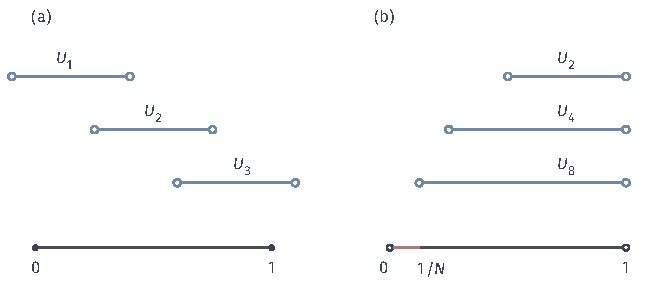
\includegraphics[width=112mm]{figures/01-mathematical-preliminaries-upper/01-mathematical-language-combinatorics-analysis-optimization/tikz/chapter3-concept-processes/finite-open-cover.pdf}
 \caption{(a) 三个开区间$(-0.1,0.4)$、$(0.25,0.75)$、$(0.6,1.1)$覆盖$[0,1]$。(b) $U_n=(1/n,1)$（$n\geq2$）覆盖$(0,1)$；只选有限多个时，设最大下标为$N$，红段$(0,1/N]$仍未覆盖。图只画$U_2,U_4,U_8$；右侧的失败由最大下标论证，不是有限图像的猜测。}
 \label{fig:analysis-process-finite-open-cover}
\end{figure}

\FloatBarrier
